% Define document class
\documentclass[modern]{aastex631}

% Import showyourwork
\usepackage{showyourwork}

% Other imports
\usepackage{listings}
\usepackage{hyperref}
\usepackage{enumitem}

% Colors
\definecolor{fancyblue}{rgb}{0.09,0.35,0.53}
\colorlet{lsthilite}{fancyblue}

% Code snippet styling
\lstdefinestyle{bash}{%
    basicstyle=\ttfamily\footnotesize,
    numbers=none,
    breaklines=true,
    frame=single
}
\lstdefinestyle{yaml}{%
    basicstyle=\ttfamily\footnotesize,
    numbers=none,
    breaklines=true,
    frame=single,
    morecomment=[l][\color{fancyblue}]{\#}
}
\lstdefinestyle{Snakefile}{%
    basicstyle=\ttfamily\footnotesize,
    numbers=none,
    breaklines=true,
    frame=single,
    morecomment=[l][\color{fancyblue}]{\#}
}
\lstdefinestyle{LaTeX}{%
    basicstyle=\ttfamily\footnotesize,
    numbers=none,
    breaklines=true,
    frame=single  
}

% URL styling
\hypersetup{%
    linkcolor=fancyblue,
    citecolor=fancyblue,
    urlcolor=fancyblue
}

% List styling
\setlist[enumerate]{wide=0pt,widest=99,leftmargin=\parindent,labelsep=*}
\setlist[itemize]{wide=0pt,widest=99,leftmargin=\parindent,labelsep=*}

% Begin!
\begin{document}

% Title
\title{\showyourwork: a workflow for open source scientific articles}

% Author list
\author[0000-0002-0296-3826]{Rodrigo Luger}
\author{Others TBD}

% Abstract with filler text
\begin{abstract}
    This paper introduces \texttt{showyourwork!}, a workflow that enables the creation and distribution of fully reproducible and open source scientific articles.
\end{abstract}

% Main body with filler text
\section{Introduction}
\label{sec:intro}
As astronomical research software becomes increasingly more complex, and as research results become increasingly more interdependent, it becomes ever more challenging to ensure the validity and correctness of results published in the literature. 
Unfortunately, the current peer review system in astronomy is simply not set up to do this.
Checking all of the results in a paper would require the painstaking and methodical review of all of the paper's methods---which usually means scrutinizing all of the code used to generate the figures, tables, and other quantities in the paper. 
In practice, this is virtually impossible for three reasons:

\begin{enumerate}
    %
    \item Modern codebases can be very large and often require deep familiarity with the software to use---not to mention review them. Volunteer referees rarely have the time to invest in learning new software in order to provide a comprehensive review.
    %
    \item  Writing a paper in astronomy is rarely ever done in a linear, procedural fashion: the codebase is constantly changing, and the state of the code when (say) Figure 1 was produced may be very different from that when (say) Figure 2 was made. 
    Moreover, many results depend on the execution of lengthy pipelines with intermediate steps, each potentially requiring manual tinkering that is not always documented and may be difficult to replicate exactly.
    %
    \item The majority of astronomical code is not open source and simply cannot be vetted by third parties. 
    While there has been a marked increase in the number of open source astronomical tools in recent years (e.g., \texttt{astropy}, \texttt{exoplanet}, \texttt{emcee}, \texttt{exofast}...), most code associated with the generation of the results in individual papers is not open source; readers are often expected to take it on faith that there are no bugs in that code, or that the code works exactly as described in the text, with no pitfalls or missing details. 
    Even when the code is made publicly available, e.g., by being published on \texttt{GitHub}, it is often not documented sufficiently to enable one to execute it and reproduce the paper's results out-of-the-box. 
    And even with proper documentation, the code may require external dependencies, custom virtual environments, or access to closed-source datasets that make it difficult or impossible for a third party to replicate it.
    %
\end{enumerate}

\texttt{showyourwork!} was designed to tackle these three issues, making it easy to develop, publish, and distribute truly open and reproducible research papers in astronomy and other scientific disciplines. 
At its core, it is a command-line tool that builds papers from a set of instructions contained in a \texttt{GitHub} repository and organized into \texttt{TeX} files, figure scripts, pipeline files, and configuration/specifications files.
Every time the user pushes a new commit to \texttt{GitHub}, the article is automatically built on the cloud using \texttt{GitHub Actions} and the resulting PDF is pushed to a separate branch of the repository. 
The build step---which sets up the conda environment, generates all figures from scratch (with intelligent caching), and compiles the PDF---acts as a unit test for the paper. 
If it passes, the paper is (by definition) reproducible.

\texttt{showyourwork!} works out of the box for simple projects, in which each figure is generated by running a given script. 
But it also works for more complicated pipelines, such as projects that depend on many intermediate steps or those that require running expensive simulations on clusters. 
The workflow interfaces directly with \texttt{Zenodo}, allowing users to automatically upload the results of simulations so that expensive build steps can be bypassed on the cloud. 
In fact, most of the features under the hood are there to make the workflow as flexible and customizable as possible.

Papers that use \texttt{showyourwork!} can be reproduced by cloning the associated repository and running \texttt{showyourwork}. 
Such papers (like this one!) include clickable icons next to each of their figures linking to (1) the exact version of the script on \texttt{GitHub} used to generate them and (2) the exact version(s) of the \texttt{Zenodo}-hosted dataset(s) used in their creation.

\section{Using \showyourwork}
\label{sec:usage}

\subsection{Prerequisites}
\label{sec:usage:prereq}
\texttt{showyourwork!} requires the \texttt{conda} package manager\footnote{\url{https://www.anaconda.com/products/distribution}} and is currently tested only on Unix-like operating systems (such as Linux, Ubuntu, or MacOS).
Users must also have access to a \texttt{GitHub} account; other \texttt{git} platforms are not currently supported.
Note that users do \emph{not} need a local installation of a \texttt{TeX} distribution, as \texttt{showyourwork!} uses the \texttt{conda}-managed \texttt{tectonic} package to compile articles.

\subsection{Installation}
\label{sec:usage:install}
\texttt{showyourwork!} can be installed with the \texttt{Python} package manager \texttt{pip}:\\

\noindent\begin{minipage}{\linewidth}
\begin{lstlisting}[
    style=bash
]
python -m pip install -U showyourwork
\end{lstlisting}
\end{minipage}

\noindent (recommended) or from source on \texttt{GitHub}:\\

\noindent\begin{minipage}{\linewidth}
\begin{lstlisting}[
    style=bash
]
git clone https://github.com/showyourwork/showyourwork
cd showyourwork
python -m pip install .
\end{lstlisting}
\end{minipage}

\subsection{Reproducing an article}
\label{sec:usage:reproduce}
Any project based on \texttt{showyourwork!} can be reproduced by cloning its \texttt{GitHub} repository and running \texttt{showyourwork}. For example, to reproduce this paper, run:\\

\noindent\begin{minipage}{\linewidth}
\begin{lstlisting}[
    style=bash,
    otherkeywords={user,repo},
    emph={user,repo},
    emphstyle={\color{lsthilite}}
]
git clone https://github.com/showyourwork/showyourwork-paper
cd showyourwork-paper
showyourwork
\end{lstlisting}
\end{minipage}

\noindent This will set up a custom \texttt{conda} environment for the workflow, download the required datasets from \texttt{Zenodo}, build all of the figures, and generate a PDF identical to this one.

\subsection{Creating a new article}
\label{sec:usage:new}
Coming soon.

\section{Repository structure}
\label{sec:struct}
%
\begin{figure}[ht!]
    \begin{centering}
        \includegraphics[width=0.25\linewidth]{figures/tree.pdf}
        \caption{
            The basic repository structure for an open source scientific article built with \texttt{showyourwork!}.
            This figure was automatically generated from the \texttt{TikZ} code in \texttt{src/scripts/tree.tex} by specifying a custom command in \texttt{showyourwork.yml}.
        }
        \label{fig:tree}
        \script{tree.tex}
    \end{centering}
\end{figure}
%
Figure~\ref{fig:tree} shows the basic directory structure for a repository instantiated from \texttt{showyourwork-template}. 
The main components are:
\begin{itemize}
    \item \texttt{.github/workflows}: Contains configuration files for the \texttt{GitHub Actions} workflows, with instructions on how to set up the virtual environment, checkout the repository, and invoke the \texttt{showyourwork-action} to build and publish the article PDF.
    \item \texttt{src/data}: Contains programmatically generated (or downloaded) datasets and dependencies that are not tracked by \texttt{git}.
    \item \texttt{src/scripts}: Contains all of the scripts and auxiliary code needed to generate the article figures.
    \item \texttt{src/static}: Contains miscellaneous files (usually figures) that are tracked by \texttt{git}.
    These may include photographs, flowcharts, or other figures that cannot be programmatically generated.
    \item \texttt{src/tex}: Contains the article manuscript and other auxiliary \texttt{TeX} files, such as the bibliography.
    \item \texttt{Snakefile}: A file containing the rules for the \texttt{Snakemake} workflow.
    By default, it simply imports all of the rules defined in \texttt{showyourwork/workflow/Snakefile}, but users can edit this file to add new rules or customize existing rules.
    \item \texttt{environment.yml}: The \texttt{conda} environment file specifying all of the direct software dependencies of the workflow.
    \item \texttt{showyourwork.yml}: The main configuration file for the workflow, where users can specify figure and dataset dependencies, instructions for downloading datasets from \texttt{Zenodo}.
\end{itemize}

\section{Examples}
\label{sec:examples}

\begin{figure}[ht!]
    \begin{centering}
        \includegraphics[width=\linewidth]{figures/eccentricity.pdf}
        \caption{
            The effect of binary eccentricity on the detectability of a \emph{LISA} gravitational wave source; reproduced from Figure 3 in \citet{Wagg2022}. 
            This figure was automatically generated from the script \texttt{src/scripts/eccentricity.py}.
        }
        \label{fig:eccentricity}
        \script{eccentricity.py}
    \end{centering}
\end{figure}

\begin{figure}[ht!]
    \begin{centering}
        \includegraphics[width=\linewidth]{figures/luhman16b.pdf}
        \caption{
            16 \emph{CRIRES} spectra of WISE 1049-5319B spanning a full rotation period of the brown dwarf; adapted from Figure 14 in \citet{Luger2021} and based on data from \citet{Crossfield2014}.
            This figure was automatically generated from the script \texttt{src/scripts/luhman16b.py} and a dataset downloaded from \texttt{Zenodo}.
        }
        \label{fig:luhman16b}
        \script{luhman16b.py}
    \end{centering}
\end{figure}

\begin{figure}[ht!]
    \begin{centering}
        \includegraphics[width=\linewidth]{figures/two_moons.pdf}
        \caption{
            A normalizing flow demonstrated on the two moons data set from \texttt{scikit-learn};
            reproduced from Figure 1 in \citet{Crenshaw2022}.
            This figure was automatically generated from the script \texttt{src/scripts/two\_moons.py}
            and an intermediate dataset that was automatically cached on \texttt{Zenodo}.
        }
        \label{fig:two_moons}
        \script{two_moons.py}
    \end{centering}
\end{figure}

\section{Integration with Zenodo}
\label{sec:zenodo}
%
Coming soon.

\section{This paper}

\begin{figure}[ht!]
    \begin{centering}
        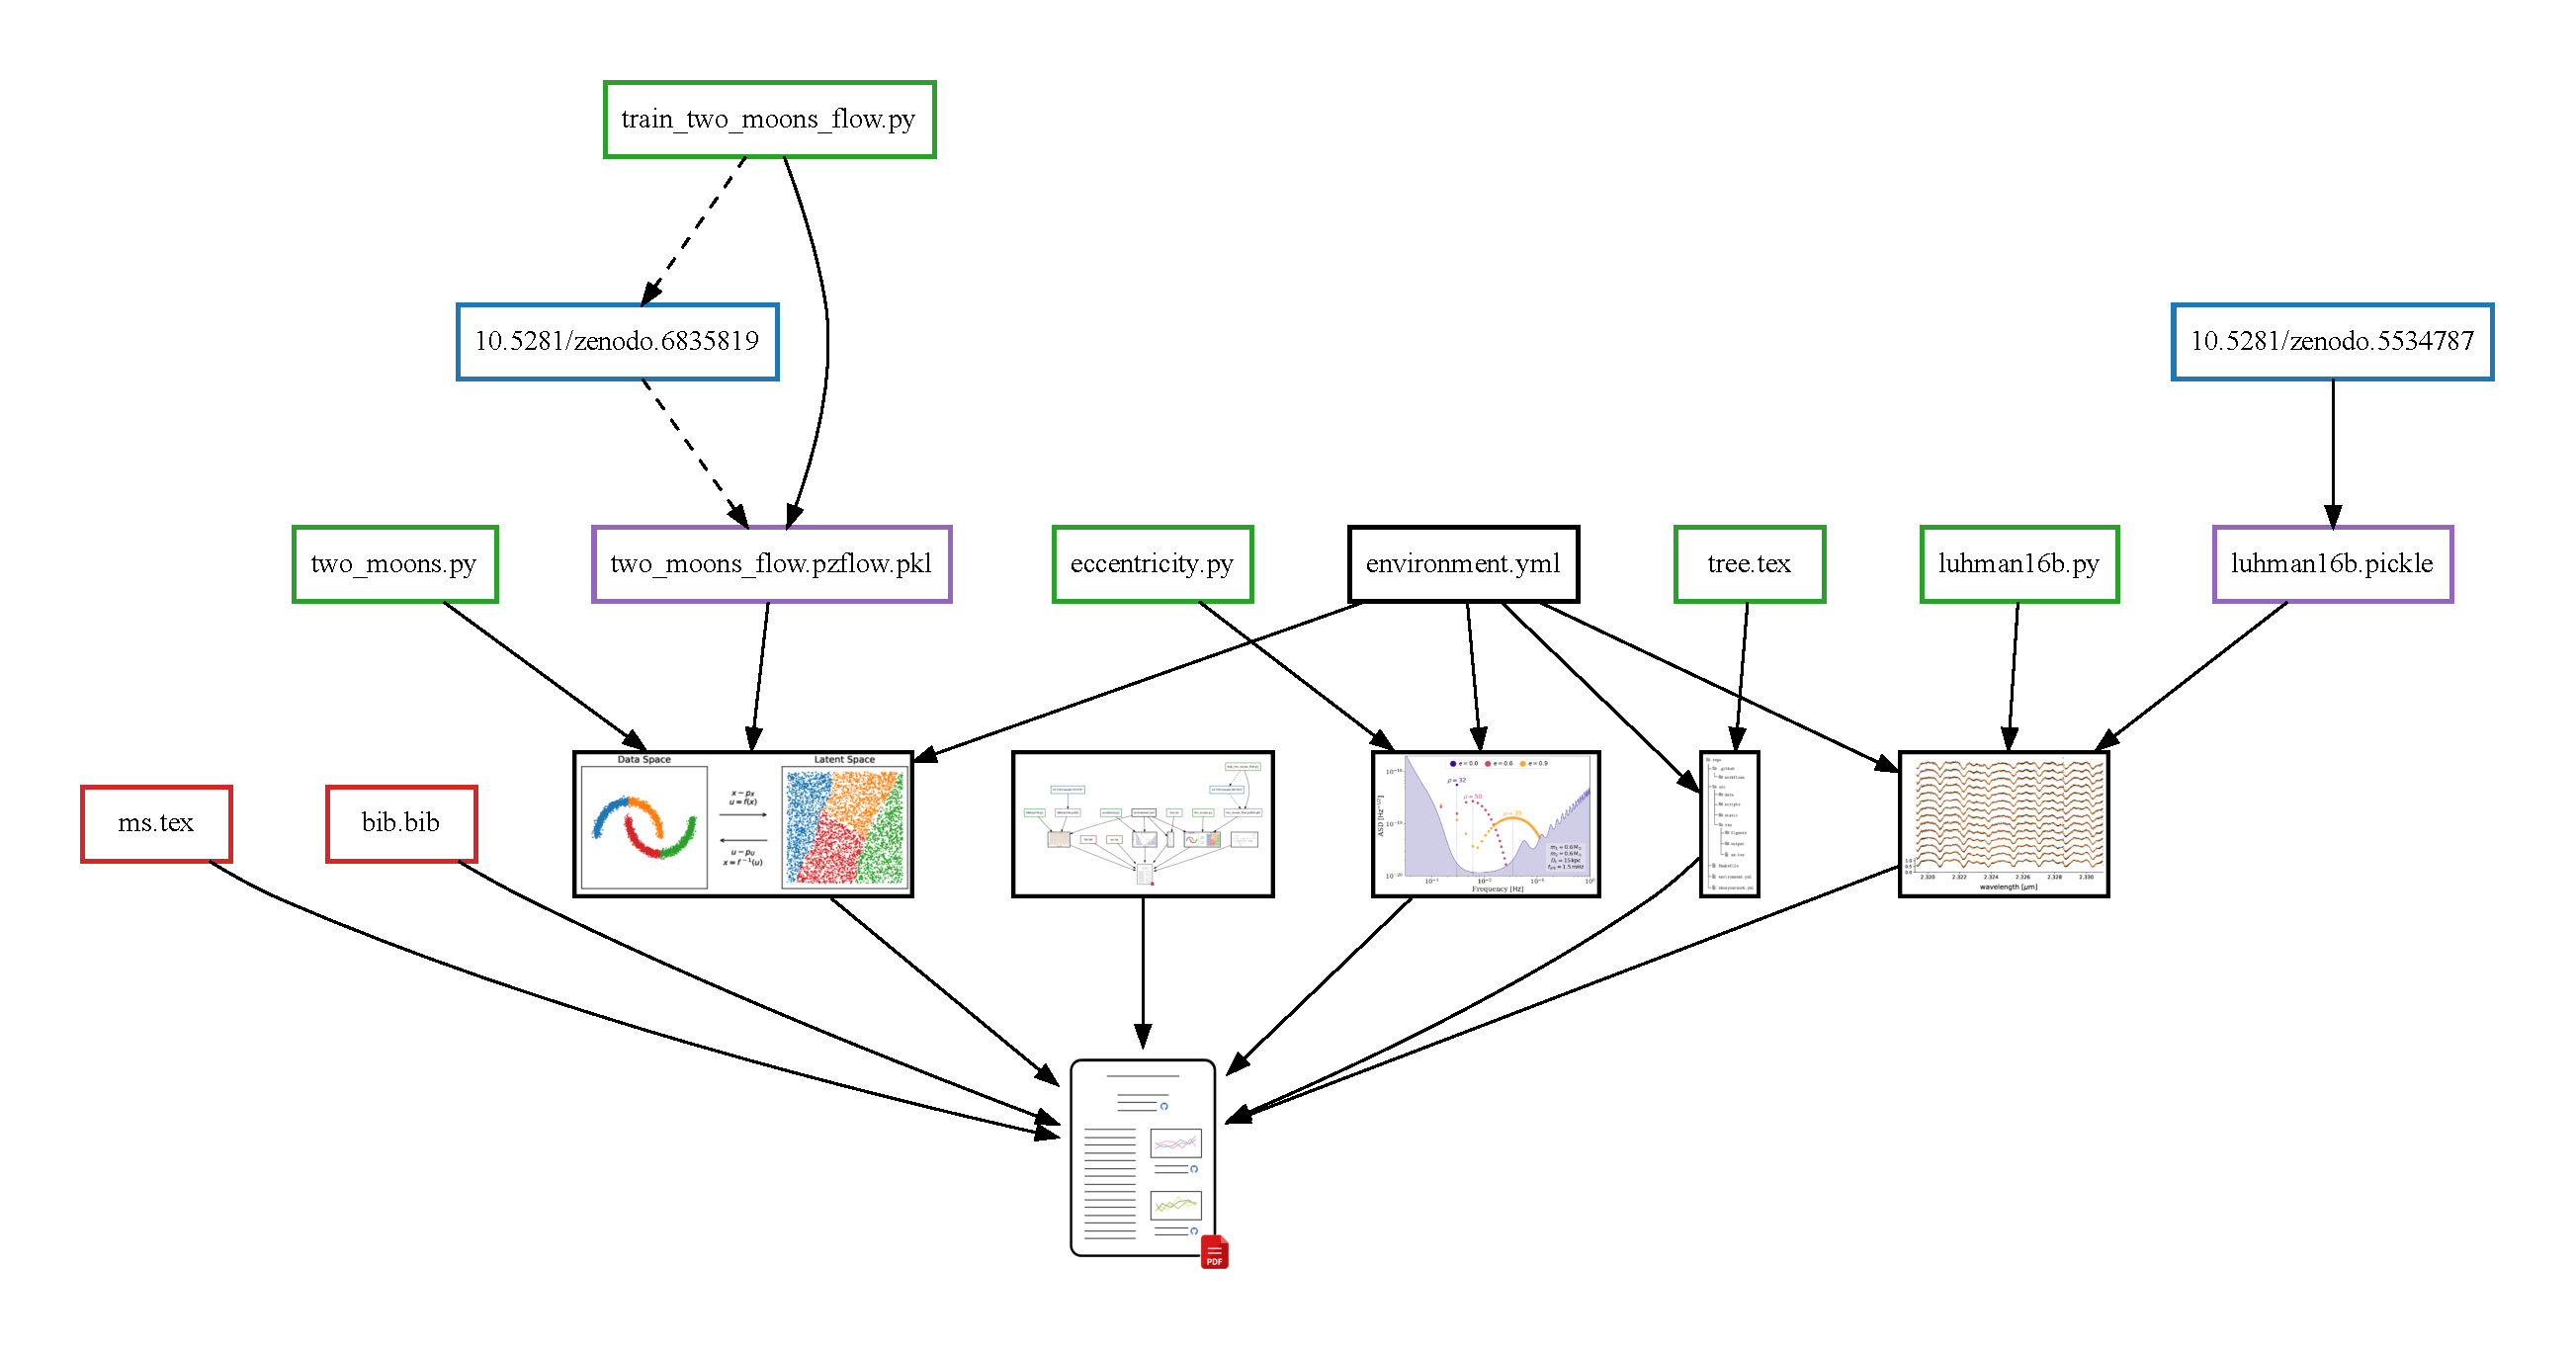
\includegraphics[width=\linewidth]{figures/dag.pdf}
        \caption{
            A directed acyclic graph (DAG) showing the complete list of dependencies for the article. 
            Scripts are shown in green, \texttt{Zenodo} deposits in blue, datasets in purple, and \texttt{TeX} files in red.
            This figure is located in the \texttt{src/static} directory and, unlike the other figures in this article, is version controlled by \texttt{git}. The \texttt{src/static} directory is reserved for figures that are not programmatically generated and simply get copied over to the output directory at compile time.
        }
        \label{fig:dag}
    \end{centering}
\end{figure}

\bibliography{bib}

\end{document}